\section{Expérimentation et Résultats}\label{Expérimentation et Résultats}
Dans cette section, nous présentons les performances de notre modèle de prédiction  du paludisme à travers une analyse des résultats des expérimentations que nous avons menées sur des jeux de données du  réelles de patients  et un jeu de données semi-synthétique obtenue  à partir du jeu de données réelles. Nous commençons par présenter les conditions d’expérimentation
\subsection{Conditions d’expérimentations}
Nous avons testé le modèle sur trois jeux de données différents en implémentant l’algorithme de la régression logistique avec le logiciel Python. Pour imputer  les données manquantes, nous avons utilisé le package missForest du logiciel R est utilisé.

\subsubsection{Nos jeux de données.} Nous avons collecté et utilisé un jeu de données patient réels provenant de différents points de santé qui ont été définis lors du Grand Magal de Touba en 2016. Nous avons également généré et utilisé deux variantes de ce jeu de données de patient réels. La description des caractéristiques de notre jeu de données brutes de patients réels, ainsi que le processus  de préparation des données que nous avions proposées pour nettoyer, normaliser et imputer les informations, sont données dans la section \ref{data_prep}. Nous notons \textsc{DT1} ce jeu de données.
La première variante, notée \textsc{DT2} est obtenue en supprimant les enregistrements avec les attributs manquants dans \textsc{DT1} au lieu d'utiliser un algorithme d'imputation qui prédit les valeurs des informations manquantes.

Une telle variante aidera à étudier l’impact de la suppression des enregistrements avec des valeurs manquantes dans l'exactitude de la prévision.
La deuxième variante, appelée \textsc{DT3}, est un jeu de données semi-synthétique qui a été généré en utilisant une stratégie de sur échantillonnage sur le jeu  de données brutes \textsc{DT1}. En effet une analyse explicative effectuée sur le jeu de données \textsc{DT1} a révélé que les données sont assez déséquilibrés, c'est-à-dire qu'il montre un déséquilibre important entre les classes; le nombre de  patients atteints de paludisme était largement inférieur au nombre de patients qui ne souffrent pas de paludisme, comme illustré à la figure \ref{records_class}. L’exploitation des approches d'échantillonnage peut permettre d’obtenir un jeu de données équilibré concernant les deux classes à prédire. 
Pour cela nous avons implémenté l’algorithme SMOTE \cite{Wa06},  avec le package \emph{imbalanced-learn} \cite{Gu17}. SMOTE consiste à créer un échantillon de données semi synthétiques à partir de la valeur dépendante  diagnostic au lieu de faire des copies des valeurs existantes. Ensuite, choisir de manière aléatoire, l'un des k plus proches voisins et l'utiliser pour créer de nouvelles observations similaires, mais au hasard.
Dossier donné afin de créer de nouvelles observations au hasard. Nous avons appliqué un sur échantillonnage de la classe minoritaire dans notre jeu de données patient pour générer un ensemble  semi-synthétique de données \textsc{DT3} contenant le même nombre d'enregistrements pour les deux classes.
% distribution of records by class
\begin{figure}[h]
\centering
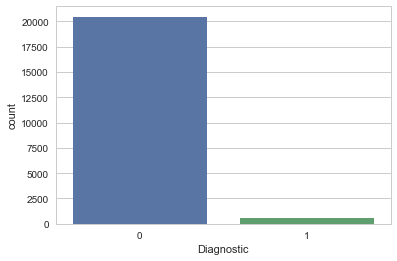
\includegraphics[width=0.6\textwidth]{images/imbalanced_dataset}
\label{records_class}\caption{The number of records by class}
\end{figure} 
% Implementation of the logistic model
\subsubsection{Paramètres du modèle de prédiction.}
 Afin de mettre en place notre modèle de classification basée sur la régression logistique, la librairie sklearn1 de Python \emph{sklearn} library\footnote{https://scikit-learn.org/stable/modules/generated/sklearn.linear\_model.LogisticRegression.html}. Ce package de python définit les paramètres par défaut de la régression logistique, ainsi que des stratégies d'optimisation, pour effectuer correctement la classification binaire en utilisant le meilleur modèle final. Pour les besoins de nos tests, nous avons utilisé les paramètres d'entrée de la régression logistique suivante
 \begin{itemize}
\item \textbf{random\_state}: modélise le l’état initial du générateur de nombres pseudo aléatoires à utiliser lors du mélange des données. Sa valeur est définie à 0 car nous n’avons pas besoin de mélanger les données dans notre expérimentation.
\item \textbf{class\_weight}: c’est le poids associés aux classes. Nous le réglons sur ‘None’, c'est-à-dire que toutes les classes sont censées avoir le poids qui est égale à 1.
\item \textbf{dual}. Il n’est mise en œuvre que pour les problèmes avec une pénalisation l2. Ce paramètre est défini sur Faux car le nombre d’échantillons est supérieur au nombre de fonctionnalités.
\item \textbf{fit\_intercept}: utile si une constante (ou biais) est ajoutée à la fonction de prédiction. Par conséquent, nous avons fixé l’interception d’ajustement à Vrai.
\item \textbf{intercept\_scaling}: ce paramètre, défini sur 1, n'est utile que lorsque le solveur «liblinear» est utilisé et fit_intercept est défini sur Vrai.
\item \textbf{max\_iter}: nombre maximum d'itérations prises pour que les solveurs convergent.
\item \textbf{multi\_class}: si l'option choisie est ovr, alors un problème binaire est correct.
\item \textbf{n\_jobs}: nombre de processeurs cpu utilisés lors de la parallélisation de classes si multi class = "ovr". Ce paramètre est ignoré lorsque le solveur est défini sur “liblinear” que «multiclass» soit spécifié ou non.

\item \textbf{penalty}: ce paramètre est utilisé pour spécifier la norme dans la pénalisation. Nous avons fixé la pénalité à sa valeur par défaut 1/2.
\item \textbf{solver}: il permet de spécifier la stratégie utilisée pour résoudre l'optimisation sous-jacente de notre modèle. Il est fixé à liblinear.
\item \textbf{tol:} tolérance pour le critère d'arrêt définie sur 0.0001.
\item \textbf{verbose}: pour le liblinear solver, définissez verbose sur un nombre positif 
\item \textbf{warm\_start}: lorsqu'il est défini sur True, réutilise la solution de l'appel précédent pour l'adapter à l'initialisation, sinon, effacez la solution précédente. Inutile pour le liblinear solver.
\end{itemize}
Comme la régression logistique effectue un apprentissage supervisé, nous avons utilisé 60\%  du jeu de données pour l’entrainement du modèle et 30\%  du jeu de données  pour  de test.
% Performance measures
\subsection{Les Mesures de performance}
Pour évaluer la performance de notre modèle de prédiction sur les différents jeux de données utilisés, nous avons calculé la précision, le rappel (ou la sensibilité), 
la F-mesure et la spécificité des classes prédites. Nous avons également tracer la courbe ROC (Receiver operating Chacacteristic) de la régression logistique pour étudier sa forme. La sensibilité, la spécificité et la courbe ROC sont souvent utilisés dans le domaine de la médecine en tant que mesure de la performance  pour l’évaluation des modèles de prédiction.
\subsubsection{Precision.}
\label{precision} . La précision p, ou taux de valeur positive, pour une classe est le nombre de vrais positifs (c’est-à-dire le nombre de cas correctement étiquetés comme appartenant à la classe \textsc{M+}) divisés par le nombre total de cas étiquetées comme appartenant à la classe \textsc{M+} (c’est-à-dire la somme des positifs et faux positifs). Les faux positifs sont les cas qui prédit dans vraies alors qu’ils  sont faux.
% precision formula
\begin{equation}
p=\frac{\sum_{i=1}^{|R|}Entity(i)}{R}.
\end{equation}
 
\textit{Entity(i)} est une fonction binaire qui renvoie true si la classe prédite pour le \textit{i}-ième cas est correct et false sinon. $R$ est la somme du nombre de vrai positifs et des faux positifs.
Recall (Rappel). Le rappel r (également appelé sensibilité) est défini comme le nombre de vrais positifs divisé par le nombre total de cas qui appartiennent réellement à la classe M + (c’est-à-dire la somme des vrais positifs et faux négatifs, qui sont des cas qui n'ont pas été étiquetés comme appartenant à la classe M + mais aurait dû être)
\subsubsection{Recall.}
% Recall formula
\begin{equation}
r=\frac{\sum_{i=1}^{\mid R\mid}Entity(i)}{G}
\label{recall}
\end{equation}
$G$est la somme du nombre de vrais positifs prédits et du nombre de faux négatifs prédits.
\subsubsection{F-measure.}la F-measure notée F$_1$, est une métrique qui mesure la précision d'un test en analyse statistique d'une classification binaire. Il est calculé en utilisant à la fois la précision $p$ et le rappel $r$ du test en tant que rapport du nombre de réponses positives et le nombre de tous les résultats positifs renvoyés par le classificateur
% F-measure formula
\begin{equation}
F_1 = 2 \times \frac{p\times r}{p + r}
\label{f-measure}
\end{equation}
\subsubsection{Specificity.}(Spécificité). La spécificité, également connue sous le nom de taux négatif réel, mesure la proportion de réels négatifs correctement identifiés en tant que tels (par exemple, le pourcentage de personnes ne souffrant pas de paludisme et qui sont correctement identifiées comme n’ayant pas la maladie).
\subsubsection{Receiver operating characteristic.}
La courbe ROC montre la capacité de diagnostic d'un système de classificateur binaire dont le seuil de discrimination est varié. La courbe ROC est obtenu en traçant le graphe \emph{vrai positif} (par exemple, sensibilité ou rappel en apprentissage automatique) par rapport au taux de faux positifs (1- spécificité) à différents seuils.
% Analysis of the results
\subsection{Expériences et analyse des résultats}
Pour chaque ensemble de données considéré, nous avons effectué deux types de tests avec notre modèle de prédiction: un test sans inclure le résultat du test de diagnostic rapide(TDR) et un autre test avec le résultat du test de diagnostic rapide (TDR) parmi les attributs d’entrée. Nous avons d'abord décrit ci-dessous les résultats obtenus pour chaque ensemble de données, puis présenté une analyse comparative
\subsubsection{Expérience avec DT1.}
Le tableau 2 et la figure 3 montrent respectivement les mesures de performance et la courbe ROC des résultats de notre approche de classification testée sur le jeu  de données DT1. Les résultats sur le tableau 2a) et la figure 3a) sont obtenus sans tenir compte du résultat de test diagnostic rapide(TDR) en contraste avec les mesures du tableau 2b) et de la figure 3b). On peut facilement voir que l'exactitude de notre modèle de prédiction est sensiblement la même lorsque l'on considère ou non le TDR; cette prédiction est assez bonne comme le prouve la précision supérieure à 90\%.
% results for precision, recall, F-measure
\begin{table}[!h]
\centering
\subtable[Prediction without the QDT outcome]{
\begin{tabular}{ccc}
\textbf{Precision} & \textbf{Recall} & \textbf{F-measure}\\
\toprule
$0.97$ & $1.0$ & $0.99$ \\
\bottomrule
\end{tabular}
}%
\hspace*{0.5cm}
\subtable[Prediction with the QDT outcome]{
\centering
\begin{tabular}{ccc}
\textbf{Precision} & \textbf{Recall} & \textbf{F-measure}\\
\toprule
$0.98$ & $1.0$ & $0.99$ \\
\bottomrule\\
\end{tabular}
}%
\label{perf-measure-dt1}\caption{Performance measures of the prediction on DT1}
\end{table}
% the roc curve
\begin{figure}[!h]
\centering
\subfigure[Prediction without the QDT outcome]{
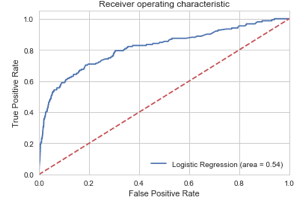
\includegraphics[width=.4\textwidth]{images/curve_roc_dt1_1}
}%
\subfigure[Prediction with the QDT outcome]{
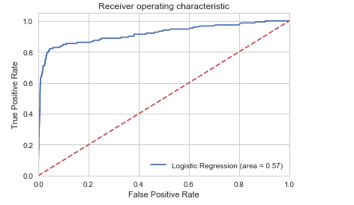
\includegraphics[width=.47\textwidth]{images/curve_roc_dt1_2}
}
\caption{The curve of the Receiver Operating Characteristic for prediction on DT1}\label{curve_roc_dt1}
\end{figure}
\subsubsection{Expériences avec DT2.}
Le tableau 3 et la figure 4 montrent respectivement les mesures de performance et la courbe ROC des résultats (avec ou sans prise en compte du TDR) de notre modèle de prédiction testée sur le jeu de données DT2. Les mesures de précision sur la table 3a) et la figure 4) respectivement à celles du tableau 3b) et de la figure 4b) montrent que notre classificateur réussit bien lorsque l'on considère le  TDR comme un attribut alors que sans le TDR la précision de la prédiction diminue.
% results for precision, recall, F-measure
\begin{table}[!h]
\centering
\subtable[Prediction without the QDT outcome]{
\begin{tabular}{ccc}
\textbf{Precision} & \textbf{Recall} & \textbf{F-measure}\\
\toprule
$0.75$ & $1.0$ & $0.86$ \\
\bottomrule\\
\end{tabular}
}%
\hspace*{0.5cm}
\subtable[Prediction with the QDT outcome]{
\centering
\begin{tabular}{ccc}
\textbf{Precision} & \textbf{Recall} & \textbf{F-measure}\\
\toprule
$1.0$ & $1.0$ & $1.0$ \\
\bottomrule
\end{tabular}
}%
\label{perf-measure-dt2}\caption{Performance measures of the prediction on DT2}
\end{table}

% the roc curve
\begin{figure}[!h]
\centering
\subfigure[Prediction without the QDT outcome]{
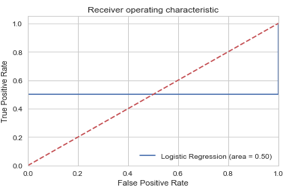
\includegraphics[width=.42\textwidth]{images/curve_roc_dt2_1}
}%
\subfigure[Prediction with the QDT outcome]{
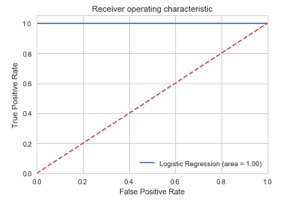
\includegraphics[width=.4\textwidth]{images/curve_roc_dt2_2}
}
\caption{The curve of the Receiver Operating Characteristic for prediction on DT2}\label{curve_roc_dt2}
\end{figure}
\subsubsection{Expériences avec DT3.}
De manière similaire aux résultats sur DT2, les mesures de performance sur DT3 montre une meilleure précision de prédiction (voir le tableau 4 et la figure 5) lorsque le TDR est pris en compte comme un attribut
% results for precision, recall, F-measure
\begin{table}[!h]
\centering
\subtable[Prediction without the QDT outcome]{
\begin{tabular}{ccc}
\textbf{Precision} & \textbf{Recall} & \textbf{F-measure}\\
\toprule
$0.77$ & $0.82$ & $0.79$ \\
\bottomrule\\
\end{tabular}
}%
\hspace*{0.5cm}
\subtable[Prediction with the QDT outcome]{
\centering
\begin{tabular}{ccc}
\textbf{Precision} & \textbf{Recall} & \textbf{F-measure}\\
\toprule
$0.87$ & $0.90$ & $0.89$ \\
\bottomrule
\end{tabular}
}%
\label{perf-measure-dt3}\caption{Performance measures of the prediction on DT3}
\end{table}

% the roc curve
\begin{figure}[!h]
\centering
\subfigure[Prediction without the QDT outcome]{
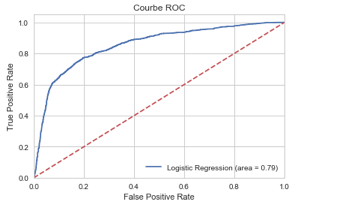
\includegraphics[width=.42\textwidth]{images/curve_roc_dt3_1}
}%
\subfigure[Prediction with the QDT outcome]{
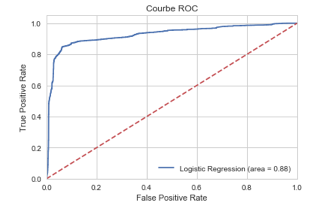
\includegraphics[width=.4\textwidth]{images/curve_roc_dt3_2}
}
\caption{The curve of the Receiver Operating Characteristic for prediction on DT3}\label{curve_roc_dt3}
\end{figure}
\subsubsection{Analyse comparative des résultats .}




